% moca.tex:

\chapter{MODULAR OPTODE CONFIGURATION ANALYZER (MOCA)} % all caps please
\label{chap:moca}

%%% Section %%% 
\section{Introduction}
\label{sec:introduction}
Functional near-infrared spectroscopy (fNIRS) is an emerging neuroimaging technique to non-invasively measure brain activity using non-ionizing light~\cite{Ferrari2012}. Unlike functional magnetic resonance imaging (fMRI)~\cite{Heinzel2013} that requires high-strength magnetic fields and large scanners, fNIRS utilizes near-infrared (NIR) light to detect brain activation by measuring the associated hemodynamics. The portability of fNIRS positions it as a competitive imaging modality to address some of the challenges of conventional neuroimaging techniques, such as fMRI and magnetoencephalography (MEG), including a lack of wearability for continuous monitoring, limited temporal resolution, and need for subject immobility during use~\cite{Yucel2017}. It has shown great promise for safe and long-term monitoring of brain activity and is increasingly used in studies for behavioral~\cite{McDonald2018} and cognitive neurodevelopment~\cite{Aslin2015, Vanderwert2014, Wilcox2015, Soltanlou2018}, language~\cite{Quaresima2012, Rossi2012}, psychiatric conditions~\cite{Ehlis2014, Kumar2017}, stroke recovery~\cite{Yang2019}, and brain-computer interfaces~\cite{Naseer2015, Ahn2017, Hong2018}. 

Despite an exponential growth in the number of applications~\cite{Boas2014, Quaresima2019} and publications~\cite{Yucel2017} in recent years, many fNIRS systems still employ fiber-based, cart-sized instrumentation~\cite{Scholkmann2014} that place limits on both channel density and the use of fNIRS in natural environments. Although fiber-based high-density~\cite{Eggebrecht2014} and portable~\cite{Wheelock2019} fNIRS systems have been demonstrated, the use of fragile fiber optics cables, stationary external source/detector units~\cite{Oxymon2017, Techen2018}, and the need for individual and specialized headgear for specific tasks have motivated the fNIRS community to investigate more flexible modular and fiber-less designs~\cite{Zhao2017, Curtin2018}.

The modular fNIRS architecture is based on utilizing elementary optical source and detector circuits (modules) as repeating building blocks to form a re-configurable probe~\cite{Zhao2017}. This modular architecture offers significantly improved portability, scalability, flexibility in coverage, and fabrication cost~\cite{Zhao2017}. By avoiding the use of fragile optical fibers, modular fNIRS systems permit the use of light guides to directly couple light sources and detectors to the scalp, significantly reducing signal loss due to fiber coupling. The lightweight and compact modules also make wearable fNIRS and continuous monitoring in mobile environments possible~\cite{Yucel2017, Park2018}. In addition, the ability to use both intra-module (within a single module) and inter-module (source and detector on different modules) channels allows for high density probes with varying source-to-detector separations (SDS) that increase measurement density and tissue depth sampling, resulting in enhanced signal quality, and easy removal of physiological noise~\cite{Gregg2010}. 

Despite these perceived benefits, the task of designing a modular fNIRS probe can quickly grow in complexity as the number of modules increases. While parameters can be empirically determined when designing a single module, understanding the trade-offs among a large array of parameters, including module shape, module size, optode quantities, and optode locations, and each parameter's effects on the final probe can become a daunting task. Not only do most published modular fNIRS studies largely focused on the design of a single module without addressing the effect of these module- and probe-level parameters on the final probe, the current literature also does not provide a means to compare probes composed of different module designs.

Aside from the challenges of determining these modular probe core parameters, other factors such as mechanical, ergonomic, safety, usability, optoelectronic, and data communication considerations~\cite{Zhao2017} also play important roles in achieving the desired performance. For example, mechanical features such as optical coupling and electronic circuitry encapsulation must be considered alongside ergonomic considerations such as comfort, weight, and robustness. Additionally, the use of high density light sources in such modular probes brings about additional safety considerations, such as heat dissipation, driving voltage, and battery life. Moreover, optoelectronic considerations arise from the use of specialized optodes with narrow emission bandwidths, high gains, low noise, and fNIRS-optimized wavelengths. Not only are these specialized optodes more expensive due to their niche applications and characteristics, they also require more complex control electronics for driving optodes and acquiring data. With such dense coverage, complex encoding strategies such as frequency~\cite{Maki1995} multiplexing become a necessity for obtaining high density data acquisition to achieve sufficient spatial and temporal resolution. Finally, while previously reported modular fNIRS systems often employ daisy-chain communication protocols to connect multiple modules on a single bus~\cite{Chitnis2016, Bci2017, Zimmermann2013, Funane2017, Zhao2019}, the design of physical inter-module connections~\cite{Zhao2021}, the synchronization method between modules~\cite{Zhao2017}, and the transfer of acquired data become increasingly complex with high module counts and branching connections.

Along these lines, a number of fNIRS data analysis packages exists~\cite{Huppert2009, Santosa2018, Hernandez2020}. However, they focus on the statistical analysis of the data ~\cite{Hernandez2020,Huppert2009, Santosa2018} to enhance its quality and provide guidance on post-processing steps such as motion artifact correction~\cite{Huppert2009}. While some other tools exist to assist in the probe design~\cite{Brigadoi2018, Machado2018, ZimeoMorais2018, Aasted2015}, most of these tools are designed to work in a highly constrained design space, where the probe parameters are mostly pre-determined by the user. As a result, the best practices and trade-offs in modular probe design such as tessellation, connection, or re-orientation are poorly explored and understood. Therefore, the community is in great need of an easy-to-use software tool to assist the exploration of and quantitative comparisons among countless parameter choices in a modular probe design and to perform a limited degree of optimization within a well-constrained configuration. 

A fully-automated probe design and optimization pipeline is impractical without application-dependent design constraints. Instead, we report a simplified, easy-to-use software toolbox to help designers navigate the vast parameter space of a modular probe. We also share a number of fundamental modular probe design strategies, discovered through our explorations via this toolbox, that are not widely recognized or previously studied. The entire workflow has been implemented into an open-source, MATLAB-based toolbox called Modular Optode Configuration Analyzer (MOCA~\cite{Vanegas2020}). MOCA supports a list of commonly used module shapes, user-defined optode layouts, and region-of-interest (ROI) coverage, and can produce quantitative performance metrics such as distributions of source-detector (SD) separations, sensitivity maps, and spatial multiplexing groupings. These performance metrics also allow comparisons between different designs of modular probes. Although MOCA is not designed as a fully-automated software that produces ``optimal'' probes regardless of application, its unique capability to describe and sweep modular probe parameters in operator-guided interrogations offers valuable perspective to start approaching the complex modular hardware design problem and make informed comparisons between well-constrained design choices.

The remainder of the paper is outlined below. In Section~\ref{sec:overview}, we discuss the relevant design considerations when developing a modular probe using MOCA. We specifically focus on the parameterization of the modules, processes required to assemble modules into functional probes, and related performance metrics for system characterization and comparisons. In Section~\ref{sec:results}, we demonstrate MOCA's capability in designing full-head probes using a variety of module shapes and compare their trade-offs regarding channel density, SD separations, and average brain sensitivities. Furthermore, we utilize MOCA to showcase potential improvements to published fNIRS probes by altering module orientations, spacing, and staggering layouts. In Section~\ref{sec:discussion}, we highlight a number of generalizable design strategies that were discovered via our experiments using MOCA, including the importance of considering module orientations, tiling strategies, and module spacing tuning, among others.



%%% Section %%%
% OVERVIEW
\section{Modular Probe Parameters and Performance Metrics}
\label{sec:overview}

\begin{figure}[ht]
    \begin{center}
    \begin{tabular}{c}
    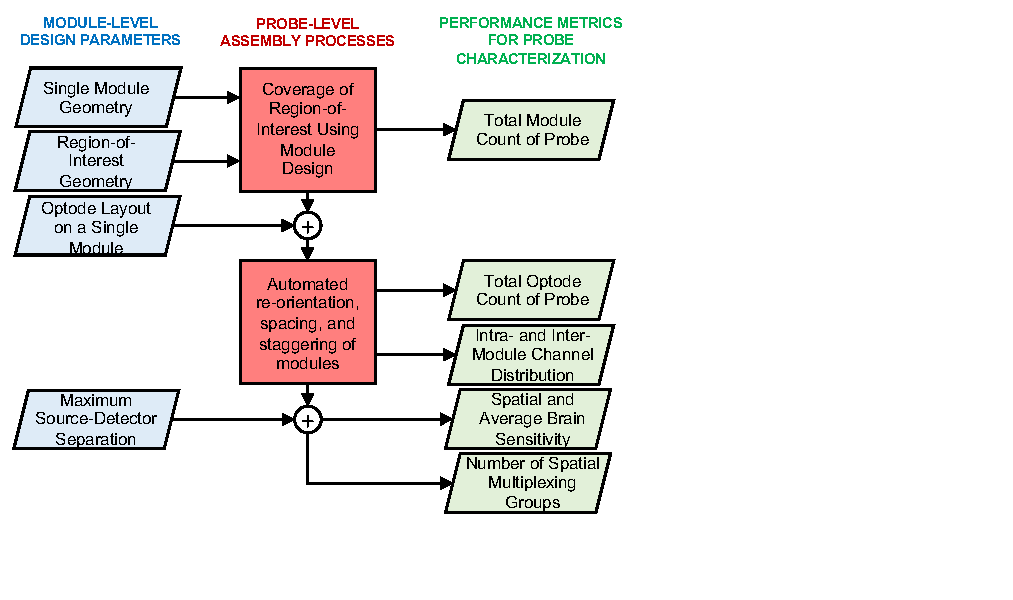
\includegraphics[height=10cm]{Fig_1.pdf}
    \end{tabular}
    \end{center}
    \caption { \label{fig:flowchart} Workflow of module-level design parameters (left column; blue) used in probe-level processes (center column; red) to produce performance metrics to characterize a probe (right column; green). Performance metrics are organized top to bottom from least complex (two parameters needed) to most complex (four parameters needed). Arrows trace how parameters are used to derive specific performance metrics.} 
\end{figure} 

A diagram showing the overall design process of a modular fNIRS system is shown in Fig.~\ref{fig:flowchart}. Specifically, the three parts describing MOCA's workflow are 1) the design parameters describing a single module design, 2) the processes and parameters used to assemble the modules into a probe, and 3) the derived performance metrics used to characterize the resulting probe. MOCA starts with the definition of essential module parameters (shown in the left column in Fig.~\ref{fig:flowchart}), applies those parameters along with probe-level constraints to a probe-generation process (center column in Fig.~\ref{fig:flowchart}), and derives quantitative performance metrics of the resulting probe (shown in the right column in Fig.~\ref{fig:flowchart}). Arrows in Fig.~\ref{fig:flowchart} define dependencies between the derived performance metrics and the input parameters. For example, in order to calculate the probe's channel distribution, one must define the module geometry, ROI, and optode layout design parameters. 

%%% Subsection %%%
\subsection{Essential module-level design parameters of fNIRS modular probes}
The basic building block of a modular probe is an fNIRS module. It is typically in the form of an optoeletronic circuit made of a rigid~\cite{Chitnis2016, Bci2017, Zhao2019, Wyser2017} or rigid-flex~\cite{Muehlemann2008, Hallacoglu2016} substrate with on-board light sources, optical sensors, auxiliary sensors, microcontrollers, and other communication electronics. A modular probe is subsequently constructed by replicating and interconnecting multiple identical modules. Therefore, the design decisions regarding the module-level parameters are highly important and directly impact the functionalities and restrictions of the resulting probe.

\subsubsection{Single module geometry}
The shape of a module is one of the key parameters when designing a modular system. In published literature, simple polyhedral shapes, especially equilateral polygons (square, hexagon, etc), are typically used due to their simplicity to fabricate, analyze, and tessellate over a target ROI. It is also possible to design probes that combine multiple polygonal shapes, such as a combination of hexagonal and pentagonal modules. Such hybrid-shape modular systems may bring advantages in tessellating curved surfaces, but they also require more complex analyses. MOCA supports a number of built-in module shapes including three equilateral polygons (triangle, square, hexagon). In such cases, the module edge length is the only shape parameter that needs to be defined. One should be aware that a small-sized module requires a large number of boards to cover a given area, thus resulting in higher fabrication cost and higher complexity in assembly and analysis. Moreover, a small module size also limits the maximum intra-module SDS. Shorter SD separations are known to be more sensitive to superficial tissues rather than brain activities. On the other hand, a small-module size provides better probe-to-scalp coupling when a rigid-board based module is used. MOCA provides support for user-specified arbitrary polygonal modules, defined by a sequence of two-dimensional (2-D) coordinates. Subsequent analyses of these user-defined arbitrary modules shapes only use the bounding box of these polygons when varying probe-level parameters.

\subsubsection{Target regions-of-interest}
An ROI refers to the area of the scalp directly above the cortex for which brain activities are expected to occur\cite{Hiroyasu2015}. For simplicity, here we focus on designing probes based on the coverage of a 2-D ROI. For generality, MOCA specifies an ROI geometry as a closed polygon made of a sequence of 2-D coordinates. Users need to specify at least three Cartesian coordinates to define a closed ROI. In the future, MOCA can potentially be expanded to support three-dimensional (3-D) surfaces as ROIs through the use of 3-D surface tessellation tools, such as the Iso2Mesh~\cite{Fang2009a} mesh generator and 3-D photon transport modeling tools such as NIRFAST~\cite{Nirfast} and Monte Carlo eXtreme~\cite{Fang2009} (MCX).

\subsubsection{Optode layout within a single module}
Optode layout refers to the spatial arrangement of optical sources and light sensors within the boundaries of a single polygonal module. In MOCA, each source and detector position is defined by a set of discrete 2-D coordinates relative to the module's center. The 2-D coordinates define the center of the active area of the light-emitting-diode (LED), laser, or photo detector. The physical dimensions of the optodes as well as the size and location of electronic components needed to drive each optode are not considered. The SD separations between all combinations of SD pairs are derived based upon the optode positions.

\subsubsection{Maximum source-detector separation and maximum short separation channel}
MOCA also considers the maximum SD separation ($SDS_{max}$) as a key design parameter. Typically, $SDS_{max}$ is determined by the signal-to-noise ratio (SNR) of the detected signal~\cite{Arnulphi2009}. A large SDS has low detector sensitivity due to the exponential decay of light intensity as SDS increases. This maximum separation limits the number inter-module channels that emerge from a particular tessellation of modules over an ROI. By default, MOCA considers any SDS below 10~mm to be a short-separation (SS) channel. This threshold can be manually changed to fit any specific optode performance or probe application. MOCA uses 30~mm as the default $SDS_{max}$~\cite{Taga2007, LloydFox2010}. MOCA bounds the SD range by the SS channel threshold and the $SDS_{max}$. 

%%% Subsection %%%
\subsection{Probe-level assembly process parameters}
A modular probe is constructed when multiple modules are arranged to form a non-overlapping coverage of the ROI area. The final probe is dependent on the tessellation (the number of modules and the spacing between them) and the orientation of each individual module in the probe.

\subsubsection{Exploring module tessellation and probe spacing}
MOCA provides a process to tessellate modules over a user-defined 2-D polygonal ROI, which is generally known as the ``tiling'' problem in computational geometry~\cite{Winslow2015}. Here, a ``complete tessellation'' refers to the tiling of an ROI using a single module shape without overlapping or leaving a gap in coverage. Each of the three built-in polygons (triangle, square, hexagon) have the ability to cover a 2-D area~\cite{Samet1990}. MOCA performs the tessellation by first tiling the module shape along a horizontal axis starting at the lowest vertical coordinate of the ROI until the width of the row composed of adjacent modules is wider than the width of the corresponding segment of ROI the row is tiled over. It then repeats this row-generation process until the height of all the rows combined is larger than the maximum height of the defined ROI. This dimension comparison in both axes accounts for module shapes with non-vertical and non-horizontal sides. For irregular module shapes, MOCA uses the maximum width and maximum height of the defined polygon as the a bounding box to create a tiling grid of the module over the ROI. Using the maximum width and height of the ROI as a guide for tiling ensures the full ROI is covered. Although MOCA offsets and flips the three equilateral polygon shapes to prevent gaps, irregular module shapes have inherent gaps between modules when tessellated. Additionally, MOCA accepts manually defined tessellations by reading a sequence of coordinates defining the center of modules to specify each individual module's location within the ROI. Following tessellation, each module is assigned a unique index and an adjacency matrix is constructed to represent which modules are next to one another.

To extend the flexibility of probe creation, users can change probe spacing, the minimum distance between adjacent modules in all directions. Additionally, a module can be manually deleted from the tessellation to allow the probe to more closely follow the boundaries of the ROI or better represent intentional empty spaces in the probe. When individual modules are removed from the probe, the adjacency matrix is re-calculated from the resulting probe. 

\subsubsection{Guiding module orientation and connection routing}
Module orientation refers to the rotation of the module along the normal direction of the ROI plane. In a ``complete tessellation'' of the three equilateral polygon shapes, MOCA appropriately flips and translates modules to prevent gaps and overlaps. For tessellations of irregular shapes, each module is simply placed in the same orientation as it was originally defined. After probe generation, MOCA allows the user to manually change the orientation of individual modules based on their assigned indices. For asymmetric optode layouts, changing the module orientation alters the SDS of inter-module channels, resulting in different performance metrics.

Additionally, MOCA creates a single sequential path to connect all modules to form a linear data communication bus, referred to as the ``routing'' process. In such a path, all modules are connected and every module is visited exactly once\textemdash a classic problem known as the Hamilton path~\cite{Kamae1967} in graph theory. In most configurations, a Hamilton path is not unique and computing such a path is known to be an NP-hard problem, i.e. problems that do not have a polynomial complexity when the node number grows. However, due to the limited module numbers commonly used in an fNIRS probes, an exhaustive search of the adjacency matrix can typically identify all Hamilton paths in a given tessellation with no more than a few minutes of computation. For any computed path, MOCA then orients each module based on the angle of a vector defined by the center of the oriented module and the center of the following module in the path. The orientation angle is relative to the horizontal axis.

%%% Subsection %%%
\subsection{Performance metrics to characterize probes}
Each metric described below changes as module- and probe-level parameters are altered either manually or through MOCA's sweeping functions. MOCA not only helps unravel the complex interplay between choices of different parameters, but also guides the probe designer in making trade-offs between conflicting design targets\textemdash improving one metric may come at the risk of worsening another. We have chosen the following set of essential performance metrics due to their ability to easily inform a breadth of end-user probe requirements such as cost, weight, depth sensitivity, and sampling rate estimates.

\subsubsection{Total module and optode counts}
Based on the module design and tessellation, MOCA computes the total number of modules, $n_m$, needed to cover the ROI. In addition, MOCA also outputs the total number of sources ($n_s$) and detectors ($n_d$) of the final probe. All modules, sources, and detectors of an assembled probe are given unique identifiable index numbers ($m_i$, $s_i$, and $d_i$, respectively). Module and optode counts are performance metrics outputted by MOCA from which cost, weight, and power estimates can be deduced.

\subsubsection{Inter- and intra-module channel distribution}
For any assembled probe, MOCA generates histograms of the SD separations for all combinations of SD pairs. Particularly, it outputs separately the distribution of inter- and intra-module channels that are below the $SDS_{max}$ previously defined by the user. These channel distributions aid the user in designing the probe based on the targeted application and population. For example shorter channels are more applicable to infant populations. Additionally, MOCA outputs channel density, a metric commonly used for fNIRS probe bench marking. Channel density is defined as the number of channels, $n_{channels}$, divided by the area of the ROI~\cite{Zhao2017}. Furthermore, MOCA can provide a spatial plot overlaying channels on the assembled probe, allowing for visual inspection of low channel density areas within the probe. 

\subsubsection{Spatial brain sensitivity}
\label{sssec:averagebrainsensitivity}
Brain sensitivity ($S_{brain}$) refers to the magnitude of the measurement signal change at a detector given a localized perturbation of optical properties of brain tissue~\cite{Strangman2013}. A higher $S_{brain}$ value suggests the probe is more sensitive to the anticipated brain activation. It is calculated from the spatial probability distribution of photons scattering through complex tissue as they travel from the source to the detector~\cite{Brigadoi2015}. Although modeling 3-D head/brain anatomies and 3-D based light simulations have been reported, including several related works from our group~\cite{Fang2009,Fang2009a,Fang2010,Brain2Mesh2020}, we deliberately chose a simplified layered-slab head model and 2-D based probe layout as default models to evaluate a modular probe in MOCA. Such a decision was largely motivated by 1) significantly faster computation and pre-/post-processing to accommodate fast sweeping of a large parameter space, and 2) avoiding another added layer of complexity when probe design is coupled with underlying brain anatomy in a 3-D head model. A comparison between $S_{brain}$ computed by 2-D and atlas based analyses is provided in the Results section. Nonetheless, MOCA can export 2-D probe data to established 3-D probe modeling toolkits, such as AtlasViewer~\cite{Aasted2015} and MCX~\cite{Fang2009}, to perform more advanced analyses when 3-D head models are necessary.

MOCA uses a five-layer slab model consisting of tissue imitating the scalp, skull, cerebral spinal fluid (CSF), white matter (WM), and gray matter (GM) to determine the spatial sensitivity profile for each SD pair in a probe~\cite{Okada2003}. The thickness of each tissue layer in the slab is set to the average thickness of that tissue type computed using the top half of a tetrahedral brain model~\cite{Sanchez2012}. We define the brain region as the combination of gray matter and white matter tissues. The optical properties and resulting thicknesses for each tissue type are summarized in Table~\ref{tab:opticalproperties}.

\begin{table}[]
\centering
\caption{Optical properties used in the slab model for calculating brain sensitivity based on Fang~\emph{et al.}~\cite{Fang2010}. The thickness of each layer is derived by dividing the total tissue volume by the tissue's surface area from a tetrahedral five tissue brain model~\cite{Sanchez2012}. The absorption coefficient, $\mu_{a}$, is the average path a photon will travel in the medium before being absorbed. Similarly, the scattering coefficient, $\mu_{s}$, defines the average path length of photons before a scattering event. Anisotropy, g, is a unit less measure of the amount of forward direction retained after a single scattering event.}
\label{tab:opticalproperties}
\begin{tabular}{@{}lcccc@{}}
\toprule
Tissue Type  & $\mu_{a}$ [$mm^{-1}$] & $\mu_{s}$ [$mm^{-1}$] & g    & Thickness [$mm$] \\ \midrule
Gray Matter                     & 0.020      & 9.000      & 0.89 & 7.25           \\
White Matter                    & 0.080      & 40.900     & 0.84 & 4.00           \\
Cerebral Spinal Fluid           & 0.004      & 0.009      & 0.89 & 2.73           \\
Skull                           & 0.019      & 7.800      & 0.89 & 3.29           \\
Scalp                           & 0.019      & 7.800      & 0.89 & 4.23           \\ \bottomrule
\end{tabular}
\end{table}

For each SD pair in the assembled probe, $3\times10^{8}$ photons are simulated using our in-house 3-D Monte Carlo photon transport simulator, MCX~\cite{Fang2009}, using a pencil beam source and a single 1.5~mm radius detector placed at the surface of the slab at its corresponding SDS. In a voxelated grid, $S_{brain}$ is defined as a ratio dividing the region-wise summation of the sensitivity matrix in each brain tissue region by the summation of the entire sensitivity matrix for each source–detector separation~\cite{Brigadoi2015}, i.e.
\begin{equation}
\label{eq:fov}
S_{brain}(s,d) = \frac{\sum_{r\in\Omega_{GM}}J(r,s,d) + \sum_{r\in\Omega_{WM}}J(r,s,d)} {\sum_{r\in\Omega}J(r,s,d)},
\end{equation}
where the sensitivity matrix, also known as the Jacobian ($J$), is computed using the adjoint Monte Carlo method~\cite{Yao2018}. In addition to $S_{brain}$, MOCA also calculates the average brain sensitivity for the entire probe, $\overline{S_{brain}}$, based on all the SD separations above the SS threshold. SS channels are excluded in the calculation of $\overline{S_{brain}}$ because, by definition, they are designed to only sample superficial layers~\cite{Brigadoi2015}.

\subsubsection{Spatial multiplexing groups}
The density of assembled modular probes may impact the probe's temporal sampling rate when illuminating each source sequentially. MOCA introduces spatial multiplexing, an encoding strategy that can potential accelerate data acquisition by simultaneously turning on multiple light sources at the same time. Because of the high attenuation of light in the head and brain tissues at large separations, MOCA can ignore the cross-talk of light sources that are far away for a given detector and assign sources into spatial multiplexing groups, or SMG, so that all sources within an SMG can be turned on simultaneously. By default MOCA uses the $SDS_{max}$ as the minimal distance between sources. This distance, however, can be defined by the user. Notably, unlike frequency multiplexing, spatial multiplexing does not require extra energy-intensive hardware or post-measurement separation of combined signals. 

The search for the SMG starts by randomly specifying a source position as the seed; a circle of radius $SDS_{max}$ centered at the seed position is drawn and a random source outside of this circle that is at least 2$\times SDS_{max}$ away is picked; the above process repeats until no additional source can be found. Once an SMG is identified, a new source that does not belong to any existing SMG is selected as the new seed for the next SMG and the above process repeats until every source is allocated. The total number of spatial multiplexing groups, $n_{SMG}$, depends on the tessellation of the module over the ROI as well as the choice of the seed position. As with channels, the $n_{SMG}$ are for a single wavelength. Thus, when estimating the total sampling rate of the probe using dual-wavelength sources, the control unit must cycle through each group twice (once for each wavelength).

In addition to $n_{SMG}$, MOCA calculates the spatial multiplexing ratio (SMR), defined as $SMR=n_s/n_{SMG}$. This ratio is interpreted as the acceleration factor of the data acquisition speed when using spatial multiplexing. For example, for a 20-source probe, an $n_{SMG}$ of 5 can accelerate the data acquisition by a factor of $SMR=20/5=4$ fold.
